\section{Validasi Hasil dan Bukti Statistik}
\label{sec:results}

Bagian ini menyajikan metodologi pengujian yang ketat dan bukti empiris dari performa \textit{Golden Model} v4.4 selama berbagai siklus pasar.

\subsection{Metodologi Pengujian}
Validasi sistem dilakukan menggunakan metode **True Walk-Forward Backtesting** dengan prinsip \textit{Zero Lookahead Bias}. Sinyal dihitung secara retrospektif hanya menggunakan informasi yang tersedia pada waktu penutupan lilin (\textit{candle close}) sebelumnya.

\subsection{Dataset dan Parameter Simulasi}
Dataset yang digunakan berasal dari data historis pasar berjangka (\textit{Futures}) Binance:
\begin{itemize}
    \item \textbf{Instrumen:} BTC/USDT Perpetual Futures.
    \item \textbf{Rentang Waktu:} Januari 2024 -- Maret 2026 (793 hari).
    \item \textbf{Frame Waktu:} 4 Jam (4H OHLCV).
    \item \textbf{Modal Awal:} \$10,000 USD.
    \item \textbf{Leverage:} 15x fixed (Notional \$15,000 per posisi).
    \item \textbf{Biaya (\textit{Fees}):} \$12 per \textit{round-trip} trade (estimasi 0.04\% taker fee).
\end{itemize}

\subsection{Performa Utama v4.4 (Langkah Jangka Panjang)}

\begin{figure}[h!]
    \centering
    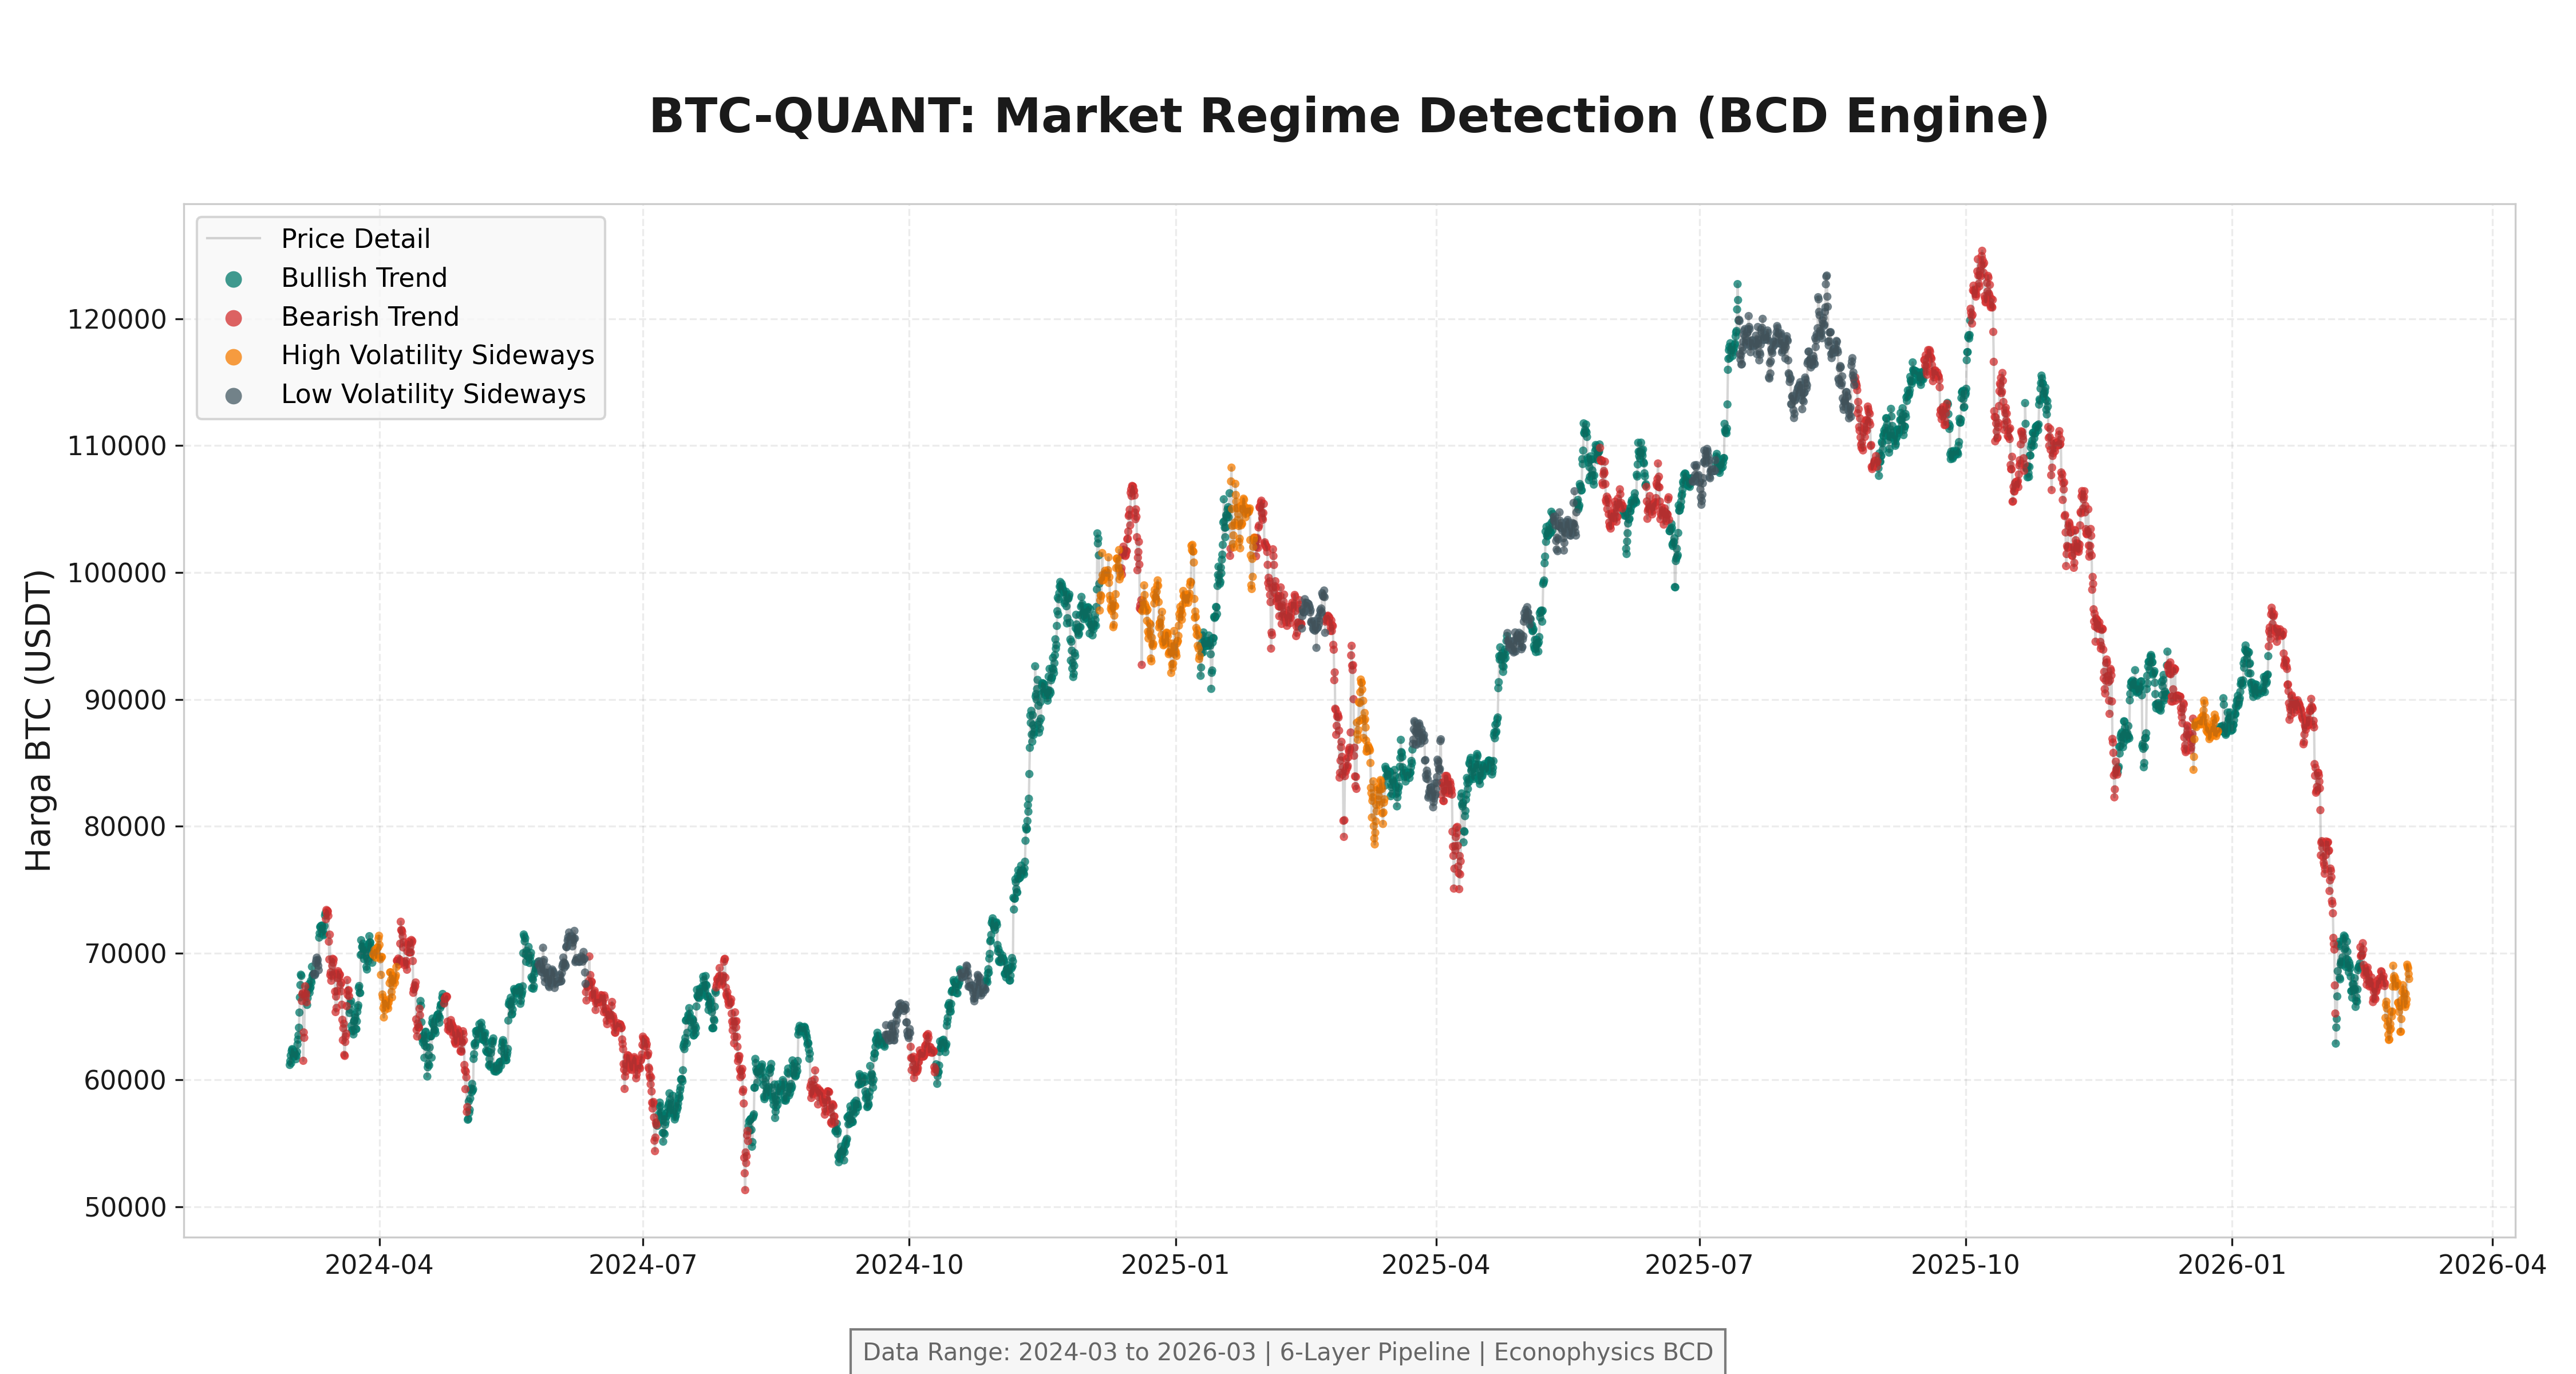
\includegraphics[width=0.9\textwidth]{figures/regime_plot.png}
    \caption{Visualisasi Plot Rezim Pasar Menggunakan Bayesian Changepoint Detection (BCD) pada Data BTC/USDT.}
    \label{fig:regime_plot}
\end{figure}

\begin{figure}[h!]
    \centering
    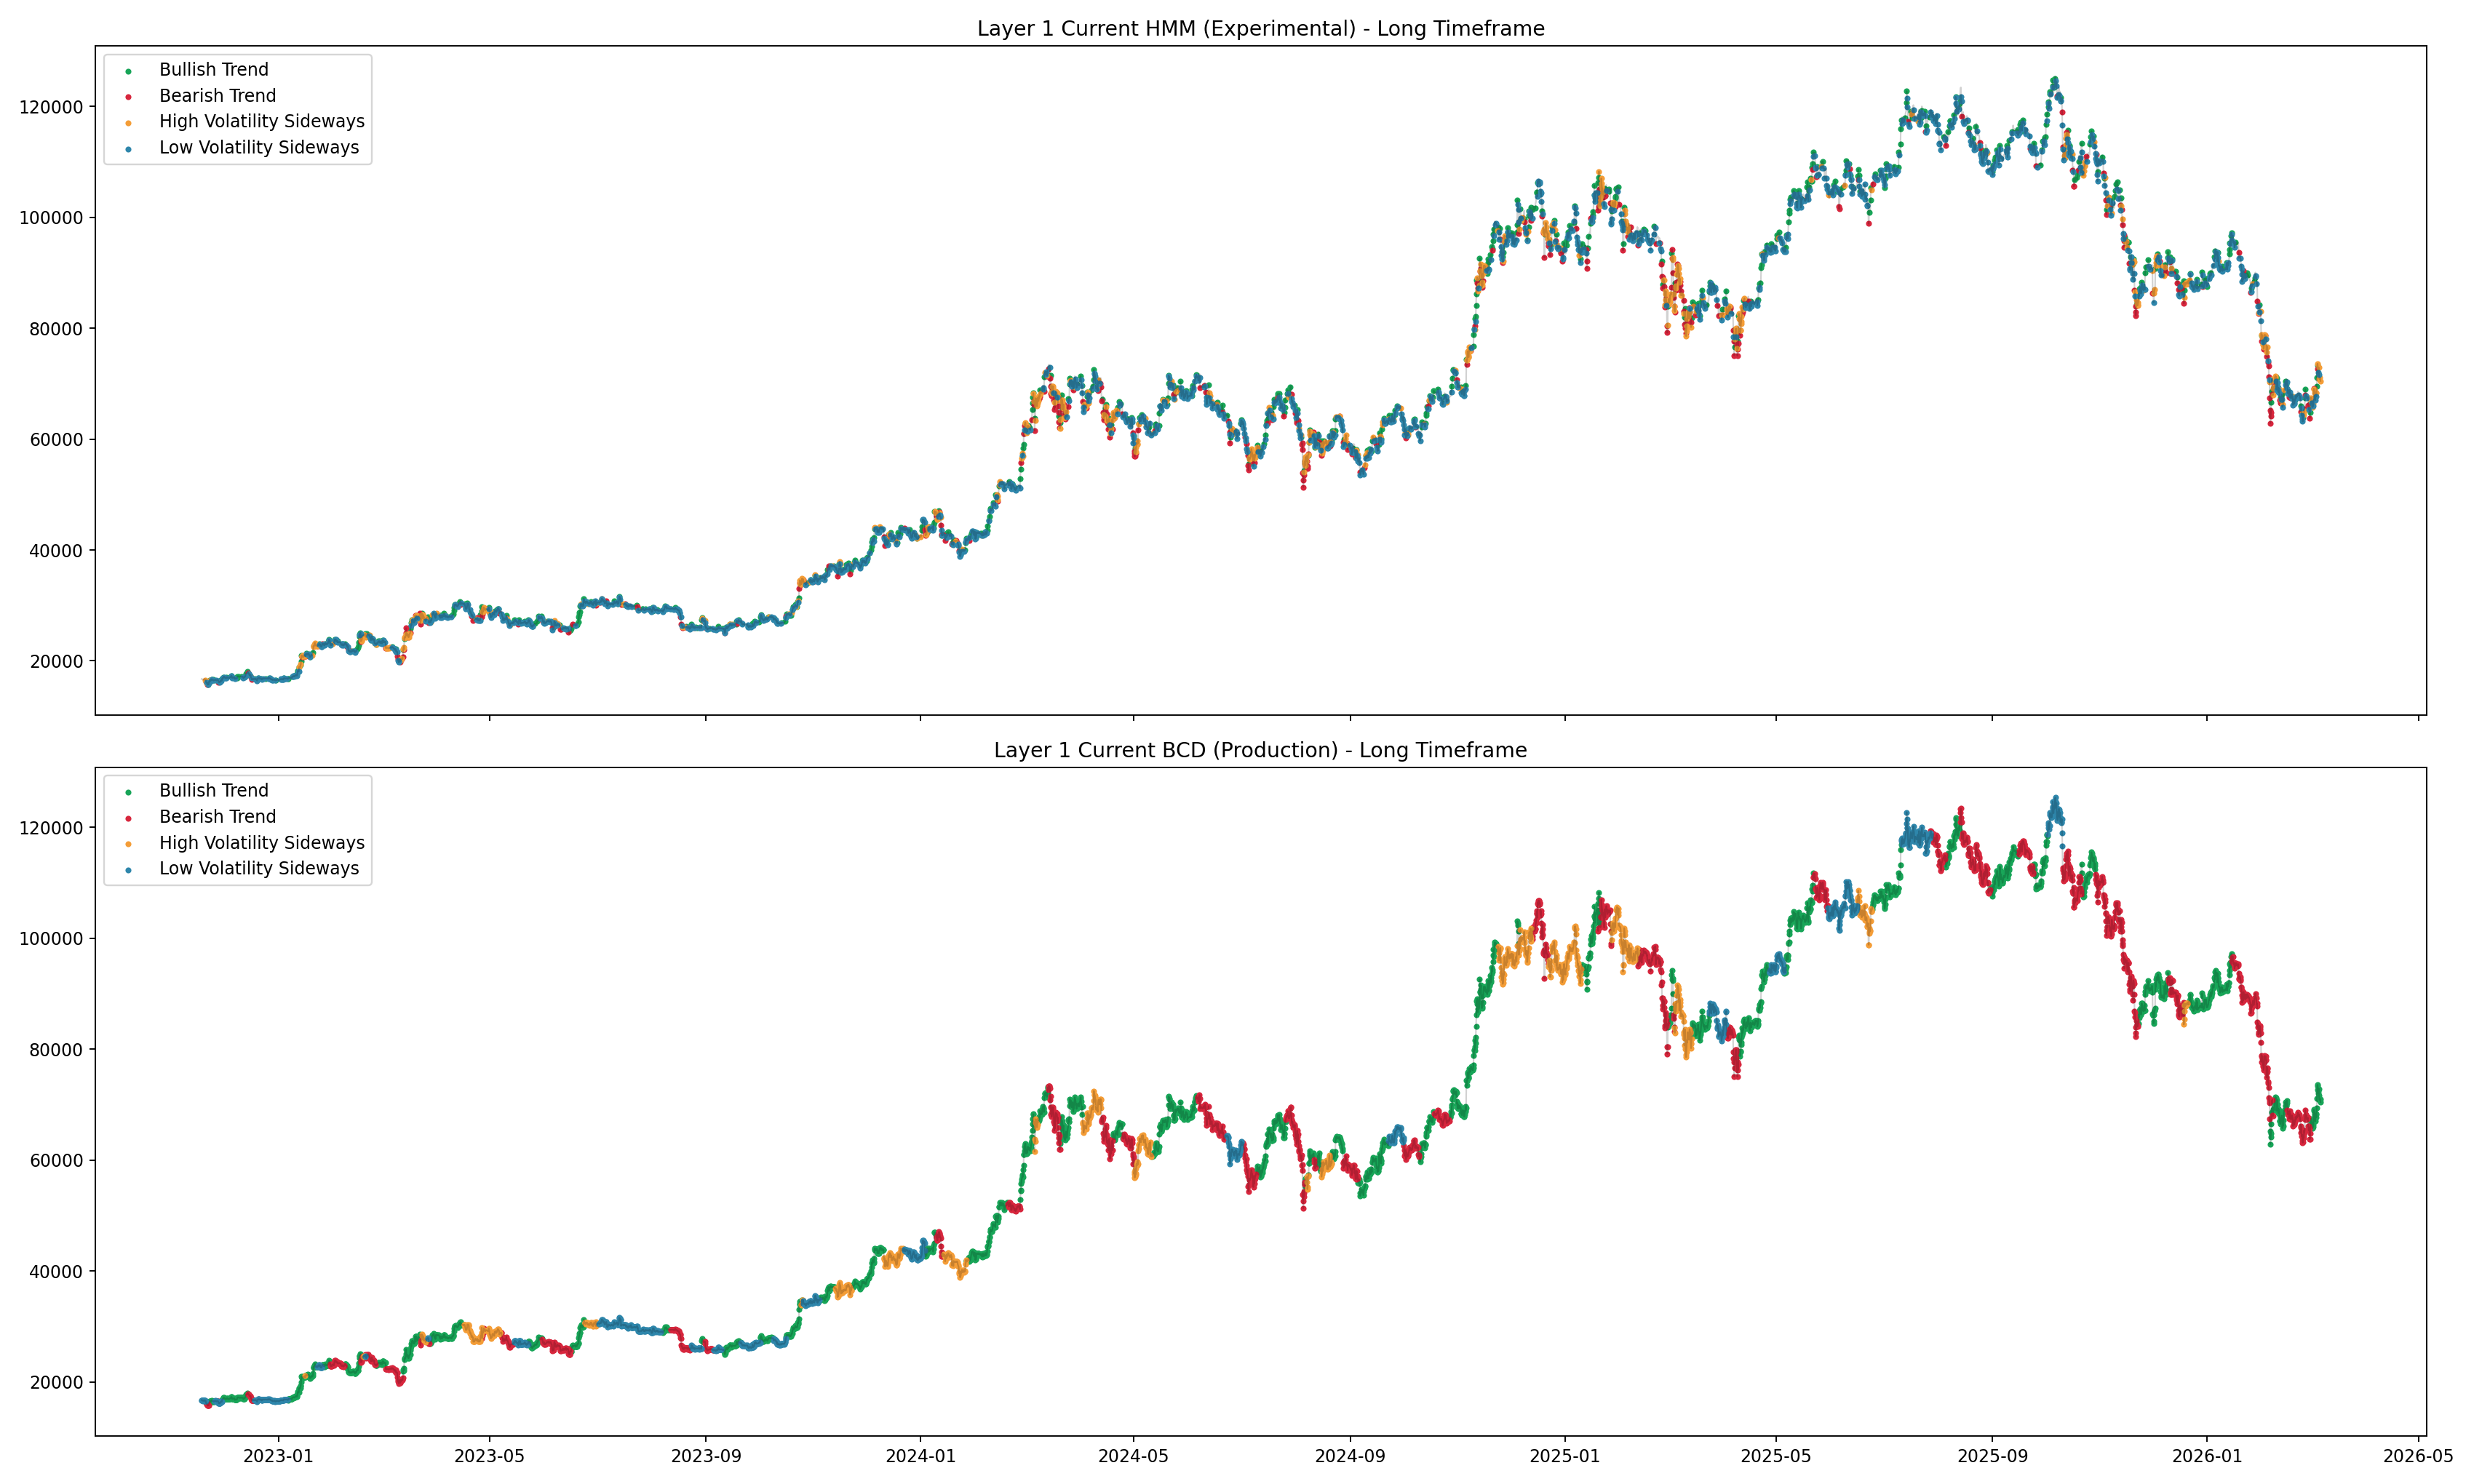
\includegraphics[width=0.9\textwidth]{figures/long_compare_viz.png}
    \caption{Perbandingan Kurva Ekuitas dan Drawdown Strategi BTC-QUANT v3 vs v4.4.}
    \label{fig:equity_comparison}
\end{figure}

Pengujian selama 793 hari membuktikan keunggulan arsitektur v4.4 dalam menjaga profil risiko yang sehat sambil tetap menghasilkan keuntungan yang konsisten.

\begin{table}[h!]
\centering
\caption{Metrik Performa Final BTC-QUANT v4.4}
\label{table:metrics}
\begin{tabular}{@{}ll@{}}
\toprule
\textbf{Metrik}          & \textbf{Nilai (v4.4)} \\ \midrule
Win Rate (WR)            & 58.07\%               \\
Net PnL (\%)             & +231.64\%             \\
Max Drawdown (MDD)       & 12.53\%               \\
Profit Factor (PF)       & 1.230                 \\
Sharpe Ratio             & 2.248                 \\
Daily Return             & 0.292\%               \\
Average Hold Time        & 11.6 jam (2.91c)      \\ \bottomrule
\end{tabular}
\end{table}

\subsection{Ketahanan Lintas Rezim Pasar}
Salah satu kekuatan utama dari pendekatan ekonofisika BCD adalah kemampuannya beradaptasi di berbagai kondisi pasar. Berikut adalah rincian performa berdasarkan deteksi rezim Layer 1 dari pengujian longitudinal 7 tahun (2019--2026, 3.866 \textit{trade}):

\begin{itemize}
    \item \textbf{Bull Market:} \textit{Win Rate} 59.9\% (2.305 \textit{trade}, kontribusi PnL +\$85.920). Memberikan kontribusi profit terbesar selama fase tren naik yang kuat.
    \item \textbf{Bear Market:} \textit{Win Rate} 56.2\% (1.561 \textit{trade}, kontribusi PnL +\$32.402). Tetap mencetak profit bersih di pasar yang menurun, membuktikan efektivitas filter arah (\textit{bias persistence}) dari Layer 1 BCD.
\end{itemize}

Konsistensi \textit{Win Rate} di atas 56\% pada kedua regime --- bahkan tanpa regime \textit{Sideways} yang terdeteksi dalam dataset 7 tahun --- mengonfirmasi bahwa \textit{Directional Spectrum} (Bab 3) secara efektif menyeleksi peluang dengan probabilitas tinggi di berbagai kondisi pasar.

% =========================================================
\subsection{Komparasi v4.4 vs Heston Adaptive v4.5: Walk-Forward 62 Hari}
\label{subsec:comparison_62d}

Sebagai lanjutan dari validasi Golden v4.4, dilakukan pengujian komparatif antara dua model secara paralel untuk mengukur dampak dari penambahan modul volatilitas adaptif Heston. Eksperimen ini dijalankan pada jendela pendek (62 hari) untuk mengisolasi performa tanpa efek compounding jangka panjang.

\textbf{Parameter Eksperimen:}
\begin{itemize}
    \item \textbf{Periode:} 1 Januari 2026 -- 4 Maret 2026 (62 hari)
    \item \textbf{Modal Awal:} \$10,000 masing-masing model
    \item \textbf{Model A (Golden v4.4):} SL tetap 1.333\%, TP tetap 0.71\%, leverage 15×, margin \$1,000/trade
    \item \textbf{Model B (Heston v4.5):} SL/TP adaptif berbasis ATR × multiplier, \textit{dynamic sizing} 2\% ekuitas/trade, leverage maks 5×
\end{itemize}

\begin{table}[h!]
\centering
\caption{Perbandingan Performa: Golden v4.4 vs Heston Adaptive v4.5 (62 Hari)}
\label{table:comparison_62d}
\begin{tabular}{@{}llll@{}}
\toprule
\textbf{Metrik}        & \textbf{Golden v4.4} & \textbf{Heston v4.5} & \textbf{Pemenang} \\ \midrule
Net PnL (\%)           & +30.04\%             & \textbf{+76.10\%}    & Heston \\
Final Equity (USD)     & \$13,004             & \textbf{\$17,610}    & Heston \\
Daily Return           & 0.485\%/hari         & \textbf{1.227\%/hari}& Heston \\
Win Rate               & \textbf{57.36\%}     & 49.35\%              & Golden \\
Profit Factor          & 1.278                & \textbf{1.587}       & Heston \\
Max Drawdown           & 20.75\%              & \textbf{17.10\%}     & Heston \\
Sharpe Ratio           & 2.299                & \textbf{3.409}       & Heston \\
R:R Ratio              & 0.950                & \textbf{1.629}       & Heston \\
Avg Winner (USD)       & \$186.67             & \textbf{\$541.38}    & Heston \\
Jumlah Trade           & \textbf{129}         & 77                   & Golden \\
\bottomrule
\end{tabular}
\end{table}

\textbf{Verdict: Heston menang 7 dari 10 metrik.} Model adaptif menghasilkan return \textbf{2.53× lebih tinggi} dengan drawdown yang lebih kecil. Kunci keunggulan Heston terletak pada tiga mekanisme struktural: (1) R:R yang lebih baik (1.63 vs 0.95) memberikan buffer keamanan lebih besar terhadap penurunan win rate; (2) \textit{dynamic position sizing} yang membatasi kerugian per trade ke 2\% ekuitas mencegah spiral drawdown; dan (3) SL/TP adaptif berbasis volatilitas aktual menghasilkan target yang lebih realistis per kondisi pasar.

Distribusi exit mengungkap satu peringatan penting: 36.4\% trade Heston keluar via \textit{TIME\_EXIT} (vs 7.0\% Golden), menandakan bahwa TP Heston terlalu ambisius untuk kondisi \textit{Low Vol} yang mendominasi periode Jan--Mar 2026.

% =========================================================
\subsection{Validasi Longitudinal 7 Tahun: Golden v4.4 vs Heston v4.5 (2019--2026)}
\label{subsec:longitudinal_7y}

Untuk mengevaluasi ketahanan kedua model terhadap berbagai siklus pasar Bitcoin, dilakukan pengujian longitudinal penuh mencakup 7 tahun data historis mulai dari fase \textit{bear market} awal 2019, lonjakan \textit{bull market} 2020--2021, siklus koreksi 2022, hingga pemulihan 2023--2026.

\textbf{Parameter Eksperimen:}
\begin{itemize}
    \item \textbf{Periode:} 18 November 2019 -- 4 Maret 2026 (2,619 hari, 13,783 candle 4H)
    \item \textbf{Modal Awal:} \$10,000 masing-masing model
    \item \textbf{Total Sinyal Dievaluasi:} Golden 11,132 (3,866 dieksekusi, 7,266 dilewati); Heston 8,951 (2,100 dieksekusi, 6,851 dilewati)
\end{itemize}

\begin{table}[h!]
\centering
\caption{Perbandingan Performa Longitudinal: Golden v4.4 vs Heston v4.5 (2019--2026)}
\label{table:longitudinal_7y}
\begin{tabular}{@{}llll@{}}
\toprule
\textbf{Metrik}          & \textbf{Golden v4.4} & \textbf{Heston v4.5}   & \textbf{Pemenang} \\ \midrule
Final Equity (USD)       & \$128,321            & \textbf{\$16,928,244}  & Heston \\
Net PnL (\%)             & +1,183\%             & \textbf{+169,182\%}    & Heston \\
Daily Return             & 0.452\%/hari         & \textbf{64.6\%/hari}   & Heston \\
R:R Ratio                & 0.976                & \textbf{1.488}         & Heston \\
Win Rate                 & \textbf{58.43\%}     & 46.67\%                & Golden \\
Profit Factor            & \textbf{1.372}       & 1.302                  & Golden \\
Max Drawdown             & \textbf{12.40\%}     & 71.94\%                & Golden \\
Sharpe Ratio             & \textbf{3.087}       & 1.007                  & Golden \\
Avg Winner (USD)         & \$193                & \textbf{\$74,481}      & Heston \\
Avg Loser (USD)          & \textbf{\$198}       & \$50,066               & Golden \\
Jumlah Trade             & 3,866                & 2,100                  & -- \\
Avg Hold Time            & 2.69 candle          & 4.30 candle            & -- \\
\bottomrule
\end{tabular}
\end{table}

\textbf{Verdict: Golden menang 6 dari 10 metrik.} Hasil ini tampak paradoks --- Heston menghasilkan ekuitas akhir \textbf{131× lebih besar} (\$16.9 juta vs \$128 ribu), namun kalah dalam metrik kualitas. Penjelasannya adalah efek \textit{compounding agresif} selama 7 tahun: setiap kemenangan Heston meningkatkan basis modal untuk trade berikutnya, menghasilkan pertumbuhan eksponensial.

Namun, keunggulan nominal ini datang dengan biaya yang signifikan:
\begin{itemize}
    \item \textbf{Max Drawdown 71.94\%} -- Pada titik terburuk, ekuitas Heston bisa menyusut hingga 72\% dari puncaknya. Sebuah akun \$16.9 juta bisa turun menjadi \$4.7 juta. Secara psikologis dan operasional, kondisi ini hampir mustahil dipertahankan tanpa intervensi.
    \item \textbf{Sharpe Ratio 1.007} -- Mendekati ambang batas minimum yang dapat diterima ($>$1.0). Return tinggi namun volatilitas yang ekstrem mengikis nilai risk-adjusted return.
    \item \textbf{TIME\_EXIT Rate 39.5\%} -- Hampir 4 dari 10 trade keluar via timeout (vs 5.4\% Golden). TP Heston yang adaptif terlalu ambisius untuk kondisi pasar rata-rata selama 7 tahun data.
    \item \textbf{High Vol Regime: Tidak Teruji} -- Seluruh 2,100 trade Heston dikategorikan sebagai regime \textit{Normal} atau \textit{Low Vol}. Multiplier SL/TP untuk kondisi \textit{High Vol} (×2.0/×1.5) sama sekali belum divalidasi secara empiris.
\end{itemize}

\begin{table}[h!]
\centering
\caption{Distribusi Exit: Golden v4.4 vs Heston v4.5 (2019--2026)}
\label{table:exit_dist_7y}
\begin{tabular}{@{}lllll@{}}
\toprule
\textbf{Exit Type} & \textbf{Golden (n)} & \textbf{Golden (\%)} & \textbf{Heston (n)} & \textbf{Heston (\%)} \\ \midrule
Stop Loss (SL)     & 1,446 & 37.4\% & 693  & 33.0\% \\
Trailing TP        & 1,261 & 32.6\% & 300  & 14.3\% \\
Full TP            & 952   & 24.6\% & 278  & 13.2\% \\
\textbf{TIME\_EXIT}& \textbf{207}   & \textbf{5.4\%}  & \textbf{829}  & \textbf{39.5\%} \\
\bottomrule
\end{tabular}
\end{table}

\begin{table}[h!]
\centering
\caption{Performa per Regime Pasar: Golden v4.4 vs Heston v4.5 (2019--2026)}
\label{table:regime_7y}
\begin{tabular}{@{}lllll@{}}
\toprule
\textbf{Model} & \textbf{Regime} & \textbf{Trades} & \textbf{Win Rate} & \textbf{Total PnL (USD)} \\ \midrule
Golden v4.4    & Bull            & 2,305           & 59.9\%            & +\$85,920 \\
Golden v4.4    & Bear            & 1,561           & 56.2\%            & +\$32,402 \\
Heston v4.5    & Bull            & 1,263           & 48.2\%            & +\$8,547,079 \\
Heston v4.5    & Bear            & 837             & 44.3\%            & +\$8,371,165 \\
\bottomrule
\end{tabular}
\end{table}

\subsubsection{Interpretasi Komparatif Lintas Horison Waktu}

Perbandingan dua horison waktu --- 62 hari vs 7 tahun --- menghasilkan kesimpulan yang saling melengkapi:

\begin{enumerate}
    \item \textbf{Jangka Pendek (62 hari):} Heston lebih baik di hampir semua dimensi kualitas (Sharpe, drawdown, profit factor) \textbf{dan} lebih profitable. Ini adalah kondisi ideal untuk deployment.
    \item \textbf{Jangka Panjang (7 tahun):} Keunggulan Heston dalam return nominal sangat besar (+169,182\% vs +1,183\%), tetapi kualitas metrik risk-adjusted (Sharpe, drawdown) memburuk secara drastis akibat compounding eksponensial yang memperbesar risiko seiring waktu.
    \item \textbf{Konsistensi Golden:} Golden mempertahankan Sharpe $>$3.0 dan drawdown $<$12.5\% bahkan setelah 7 tahun --- bukti stabilitas arsitektur yang tidak terdegradasi lintas siklus pasar.
\end{enumerate}

\textbf{Kesimpulan praktis:} Untuk akun produksi dengan batasan risiko institusional (drawdown $<$20\%), Golden v4.4 adalah pilihan yang lebih aman. Untuk akun eksplorasi dengan toleransi risiko tinggi dan horison panjang, Heston v4.5 menawarkan potensi return eksponensial yang belum tertandingi --- dengan catatan bahwa regime \textit{High Vol} masih merupakan \textit{blind spot} yang harus divalidasi sebelum deployment penuh.
